%++++++% Preâmbulo %+++++++++++++++++++++++++++++++++++++++++++++++++++++++++
\documentclass[13pt, xcolor={dvipsnames,svgnames}, portuguese]{beamer}
%\documentclass[[11pt, xcolor={dvipsnames,svgnames,table},portuguese]{beamer} 

\usetheme{CambridgeUS}

\setbeamercolor*{structure}{bg=PineGreen!20,fg=PineGreen} %fg=PineGreen
\definecolor{beamer@pinegreen}{rgb}{0.137,0.666,0.741}


\setbeamercolor*{palette primary}{use=structure,fg=white,bg=structure.fg}
\setbeamercolor*{palette secondary}{use=structure,fg=white,bg=structure.fg!75}
\setbeamercolor*{palette tertiary}{use=structure,fg=white,bg=structure.fg!50!black}
\setbeamercolor*{palette quaternary}{fg=white,bg=black}

\setbeamercolor{section in toc}{fg=black,bg=white}
\setbeamercolor{alerted text}{use=structure,fg=structure.fg!50!black!80!black}

\setbeamercolor{titlelike}{parent=palette primary,fg=structure.fg!50!black}
\setbeamercolor{frametitle}{bg=gray!10!white,fg=PineGreen}

\setbeamercolor*{titlelike}{parent=palette primary}

\usepackage[utf8]{inputenc}
\usepackage[brazil]{babel}  % idioma
\usepackage{amsmath,amsfonts,amssymb,textcomp}
\usepackage{graphicx}
\usepackage{subfigure}
\usepackage[utf8]{inputenc}
\usepackage{ifpdf}
\usepackage{listings}

% Configurações para o ambiente lstlisting
\lstset{
    language=C,
    basicstyle=\ttfamily\footnotesize,
    numbers=left,
    numberstyle=\tiny,
    numbersep=5pt
}

% here you should include other packages with \usepackage

    \ifpdf

      % hyperref should be the last package loaded:
	  %\usepackage[pdftex]{hyperref}
      \usepackage{pst-pdf}
    \else

      % make the command \href from hyperref available as a 'print only'
      \newcommand{\href}[2]{#2}

    \fi

%Global Background must be put in preamble
\usebackgroundtemplate%
{%
    
\includegraphics[width=\paperwidth,height=\paperheight]{Figuras/fundo.png}%
}
\setbeamertemplate{frametitle}[default][center]
 
\author{Othon Oliveira}
\title{Lógica de Programação com Java Script}
\institute{SENAC - PROA} 
\date{} 
%\subject{} 

\begin{document}

\begin{frame}
\titlepage
%\date{}
\end{frame}

% Capa - requer o TikZ
\newcommand{\capa}{
    \begin{tikzpicture}[remember picture,overlay]
        \node at (current page.south west)
            {\begin{tikzpicture}[remember picture, overlay]
                \fill[shading=radial,top color=orange,bottom color=orange,middle color=yellow] (0,0) rectangle (\paperwidth,\paperheight);
            \end{tikzpicture}
          };
    \end{tikzpicture}
}

\begin{frame}\frametitle{Sumário}
\tableofcontents
\end{frame}

%++++++++++++++++++++++++++++++++++++++++++++++
\section{Estudo de funções em JavaScript}
%++++++++++++++++++++++++++++++++++++++++++++++
\begin{frame}[fragile]
\frametitle{Introdução às Funções}

\begin{itemize}
  \item Uma função é um bloco de código reutilizável projetado para realizar uma tarefa específica.
  \item Funções podem aceitar parâmetros (dados de entrada) e podem retornar um valor.
\end{itemize}

\end{frame}
%----------------------------------------------
\begin{frame}[fragile]
\frametitle{Como funcionam as Funções}
\begin{center}
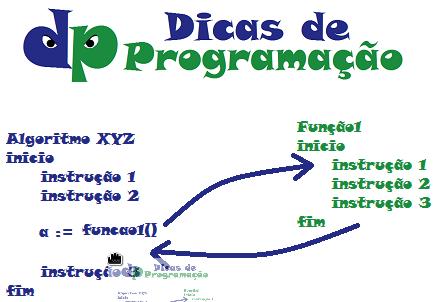
\includegraphics[scale=0.5]{Figuras/funcao.png}
\end{center}
\end{frame}
%----------------------------------------------

\begin{frame}[fragile]
\frametitle{Sintaxe de Declaração de Função}

\begin{verbatim}
function nomeDaFuncao(parametro) {
  // Código da função
}

const nomeDaFuncao = function(parametro) {
  // Código da função
};

\end{verbatim}

\end{frame}
%---------------------------------------------
\begin{frame}[fragile]
\frametitle{Exemplo de Função com Parâmetro}

\begin{verbatim}
function saudacao(nome) {
  console.log(`Olá, ${nome}!`);
}

saudacao("Alice"); // Saída: Olá, Alice!
saudacao("Bob");   // Saída: Olá, Bob!
\end{verbatim}

\end{frame}
%---------------------------------------------
\begin{frame}[fragile]
\frametitle{Exemplo de Função com Retorno}

\begin{verbatim}
function calcularQuadrado(numero) {
  return numero * numero;
}

const resultado = calcularQuadrado(5); // resultado é 25
\end{verbatim}

\end{frame}
%---------------------------------------------
\begin{frame}[fragile]
\frametitle{Funções como Parte de Expressões}

\begin{itemize}
  \item Funções também podem ser usadas como parte de expressões.
  \item Elas podem ser atribuídas a variáveis e passadas como argumentos para outras funções.
\end{itemize}

\end{frame}
%----------------------------------------------
\begin{frame}[fragile]
\frametitle{Funções como Parte de Expressões - Exemplo "Simples"}

\begin{verbatim}
const saudacao = function(nome) {
  return `Olá, ${nome}!`;
};

// usando a função "saudação
const mensagem = saudacao("Eva");
console.log(mensagem); // Saída: Olá, Eva!
\end{verbatim}

   \begin{itemize}
     \item A função saudacao é atribuída a uma variável como uma expressão de função anônima.
     \item Essa função aceita um parâmetro nome e retorna uma saudação personalizada.
     \item A variável mensagem armazena o resultado da chamada da função saudacao.
	\end{itemize}

\end{frame}
%----------------------------------------------

%----------------------------------------------
\begin{frame}[fragile]
\frametitle{Funções como Parte de Expressões - Exemplo "Sofisticado"}

\begin{verbatim}
const multiplicador = function(fator) {
  return function(numero) {
    return numero * fator;
  };
};

const duplicar = multiplicador(2);
const triplicar = multiplicador(3);

console.log(duplicar(5)); // Saída: 10
console.log(triplicar(5)); // Saída: 15
\end{verbatim}
    A função multiplicador é uma função de ordem superior que retorna uma função.
    A função retornada multiplica um número pelo fator passado na primeira função.
    As variáveis duplicar e triplicar armazenam funções de multiplicação por 2 e 3, respectivamente.

\end{frame}

%-----------------------------------------------
\begin{frame}[fragile]
\frametitle{Exercícios de Funções em JavaScript}

\begin{itemize}
  \item Exercício 1: Somar Dois Números
  \item Exercício 2: Verificar Número Par
  \item Exercício 3: Calcular Média
  \item Exercício 4: Converter Polegadas para Centímetros
  \item Exercício 5: Verificar Triângulo
  \item Exercício 6: Calcular Área do Triângulo
  \item Exercício 7: Verificar Maior Número
  \item Exercício 8: Calcular Desconto
  \item Exercício 9: Verificar Número Primo
  \item Exercício 10: Calcular Fatorial
\end{itemize}

\end{frame}

\begin{frame}[fragile]
\frametitle{Exercício 1: Somar Dois Números (HTML/JavaScript) Parte 1}

\begin{verbatim}
<!DOCTYPE html>
<html>
<head>
  <title>Exercício 1: Somar Dois Números</title>
</head>
<body>
  <h1>Exercício 1: Somar Dois Números</h1>
  <script>
    function somar(a, b) {
      return a + b;
    }
\end{verbatim}

\end{frame}
%-----------------------------------------------
\begin{frame}[fragile]
\frametitle{Exercício 1: Somar Dois Números (HTML/JavaScript) Parte 2}

\begin{verbatim}
    const num1 = parseFloat(prompt("Digite o primeiro número:"));
    const num2 = parseFloat(prompt("Digite o segundo número:"));

    const resultado = somar(num1, num2);
    document.write(`A soma é: ${resultado}`);
  </script>
</body>
</html>
\end{verbatim}

\end{frame}

%+++++++++++++++++++++++++++++++++++++++++++++++
\section{Entrada - processamento e saída }
\subsection{Praticando com JavaScript e HTML}
%+++++++++++++++++++++++++++++++++++++++++++++++
\begin{frame}
\frametitle{Cálculo do Valor da Conta em um bar}

Cinco amigos combinaram de ir a um bar tomar chopp.\\
O bar dá desconto (happy hour) até às 19h, sendo que somente 2 amigos do grupo conseguiram chegar ao bar antes das 19h e tomaram 4 chopps cada.\\
O desconto é não cobrar os 10\%
O restante do grupo chegou após o happy hour e não conseguiram mais o desconto.\\
Elaboe um algoritmo em JavaScript que calcule o valor dessa conta.\\
Exiba um formulário em HTML no qual um garçon insira os produtos e emida um relatório (em HTML) com a conta final a ser paga.

\end{frame}


\begin{frame}
\frametitle{Cálculo do Valor da Conta em um Restaurante}

\begin{itemize}
  \item Calcule o valor total da conta.
  \item Calcule a taxa de serviço de 10%.
  \item Adicione a taxa de serviço ao valor total.
  \item Exiba o valor final a ser pago.
\end{itemize}

\end{frame}
%-------------------------------------------------------------
\begin{frame}
\frametitle{Cálculo do Valor da Conta - Exemplo}

\begin{block}{Passo 1}
Digite o valor e a quantidade antes do happy hour (4 chopps)
\end{block}

\begin{block}{Passo 2}
Digite o valor e a quantidade após o happy hour (6 chopps)
\end{block}


\begin{block}{Passo 3}
Calcule a taxa de serviço (10\%) Ex.: $0.10 \times 150.00 = \textbf{R\$ 15.00}$
\end{block}

\begin{block}{Passo 4}
Adicione a taxa de serviço ao valor total:\\
Exemplo: $150.00 + 15.00 = \textbf{R\$ 165.00}$
\end{block}

\begin{block}{Passo 5}
O valor final a ser pago é \textbf{R\$ 165.00}
\end{block}

\end{frame}

%-------------------------------------------------------------
%\begin{frame}[fragile]
%\frametitle{Exemplo de Uso da Média Aritmética}
%Vamos calcular a média aritmética de um conjunto de valores.
%\begin{verbatim}
%Vamos calcular a média aritmética dos valores 10, 15, 20, 25 e 30.
%
%\begin{verbatim}
%const valor1 = 10, valor2 = 15, valor3 = 20;
%const valor4 = 25, valor5 = 30;
%
%const soma = valor1 + valor2 + valor3 + valor4 + valor5;
%const quantidade = 5;
%const media = soma / quantidade;
%
%console.log("Soma:", soma);
%console.log("Média Aritmética:", media);
%
%\end{verbatim}
%Pergunta: Onde deverei "colar" esse código, para que funcione
%do jeito que está?
%\end{frame}

%+++++++++++++++++++++++++++++++++++++++++++++++
%\section{Calculos com mais um pouco de desafios}
%+++++++++++++++++++++++++++++++++++++++++++++++

%-------------------------------------------------------------
%\begin{frame}[fragile]
%\frametitle{Exemplo de Cálculo de Juros Simples}
%
%Aqui está um exemplo de cálculo de juros simples em HTML:
%
%\begin{verbatim}
%<!DOCTYPE html>
%<html>
%<head> <title>Cálculo de Juros Simples</title> </head>
%<body>
%  <h1>Calculadora de Juros Simples</h1>
%  <script>
%    const principal = 5000;
%    const taxaDeJuros = 10; // 10%
%    const periodo = 2;
%    const montante = principal + (principal * taxaDeJuros / 100 * periodo);
%    const resultado = `Montante com Juros Simples: $${montante.toFixed(2)}`;
%    document.write(resultado);
%  </script>
%</body>
%</html>
%\end{verbatim}
%
%\end{frame}
%-------------------------------------------------------------
%\begin{frame}[fragile]
%
%
%\end{frame}

%%+++++++++++++++++++++++++++++++++++++++++++++++


%+++++++++++++++++++++++++++++++++++++++++++++++




%-----------------------------------------------

\end{document}